\section{Experimental Evaluation}
\label{sec:exp}

{\bf Experimental environment.} All experiments in this section were
conducted on an 8-slave in-house Open Stack cloud, using Linux Ubuntu
14.04 and Spark v1.4.  Each node has 4 cores and 16 GB of RAM.  Spark
Standalone cluster manager and Hadoop 2.6 were used.

Because Spark is a lazy evaluation system, a \insql{materialize}
operation was appended to the end of each query, which consisted of
the count of nodes and edges.  In cases where the goal was to evaluate
a specific operation in isolation, we used warm start, which consisted
of materializing the graph upon load.  Each experiment was conducted 3
times, we report the average running time, which is representative
because we took great care to control variability.  Standard deviation
for each measure is at or below 5\% of the mean except in cases of
very small running times.

{\bf Data.}  We evaluate performance of our framework on two real
open-source datasets.
%\begin{enumerate}%[leftmargin=*]
%\item 
DBLP~\cite{dblp} contains co-authorship information from 1936 through
2015, with over 1.5 million author nodes and over 6 million undirected
co-authorship edges.  Total data size: 250 MB.
%
nGrams~\cite{nGrams} contains word co-occurrence information from 1520
through 2008, with over 1.5 million word nodes and over 65 million
undirected co-occurrence edges.  Total data size: 40 GB.  

The nGrams dataset is of comparable size to the LiveJournal dataset
in~\cite{Xin2013} and is commensurate with our cluster size.  DBLP and
nGrams differ not only in size, but also in the evolutionary
properties: co-authorship network nodes and edges have limited
lifespan, while the nGrams network grows over time, with nodes and
edges persisting for long duration.  All figures in the body of this
section are on the larger nGrams dataset.  Refer to the Appendix for
the DBLP figures, which show similar trends as nGrams.  We plan to
carry out further experiments with a larger
DELIS\footnote{\url{law.di.unimi.it/webdata/uk-union-2006-06-2007-05}}
dataset as we grow the cluster in the near future.

\subsection{PageRank}

Snapshot analytics like PageRank are implemented using
the Pregel API in GraphX, with batch mode for MGC and OGC.  We used
the following query to evaluate data structure performance over
varying number of snapshots:

\begin{small}
\begin{verbatim}
      TSelect V[vid, pagerank()];
              E[vid1, vid2]
      From    nGrams
      TWhere  Start >= x And End <= y
\end{verbatim}
\end{small}

PageRank was executed for 10 iterations or until convergence,
whichever came first.  Performance of Pregel-based algorithms depends
heavily on the partition strategy, with best results achieved where
cross-partition communication is small.  For this reason, we evaluated
only no partitioning and E2D.

SG performs better than the other data structures in this experiment,
contrary to our expectation that batch mode of MGC and OGC would be
faster (Figure~\ref{fig:pagerank}).  This can be explained by MGC and
OGC using significantly more cross-partition communication due to the
following factors:

\begin{enumerate}[leftmargin=*]
\item Each individual snapshot is less dense than the aggregate
  (although this depends on the rate of change), and dense graphs do
  worse with Pregel analytics.
\item Individual snapshots are smaller and take fewer partitions, so
  less communication happens across partitions.
\item PageRank gets faster as vertex values converge, because those
  vertices stop sending out new messages.  In OGC/MGC a vertex converges
  only when it does so in all snapshots.
\eat{\item Messages for OGC are larger --- it is more costly to send a Map
  object than a number.}
\end{enumerate}

\begin{figure*}[t]
\centering
\begin{minipage}{3in}
  \centering
  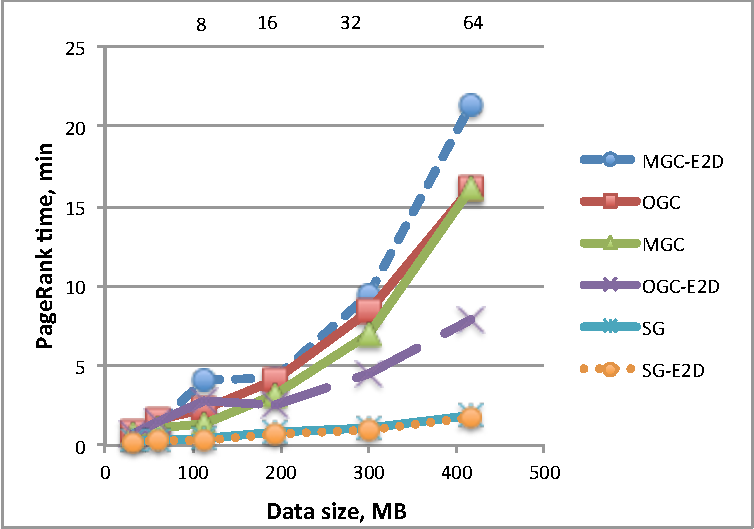
\includegraphics[width=2.6in]{figs/pagerank.pdf}
  \vspace{-0.1in}
  \caption{PageRank time.}
  \label{fig:pagerank}
  \vspace{-0.1in}
\end{minipage}
\begin{minipage}{3in}
  \centering
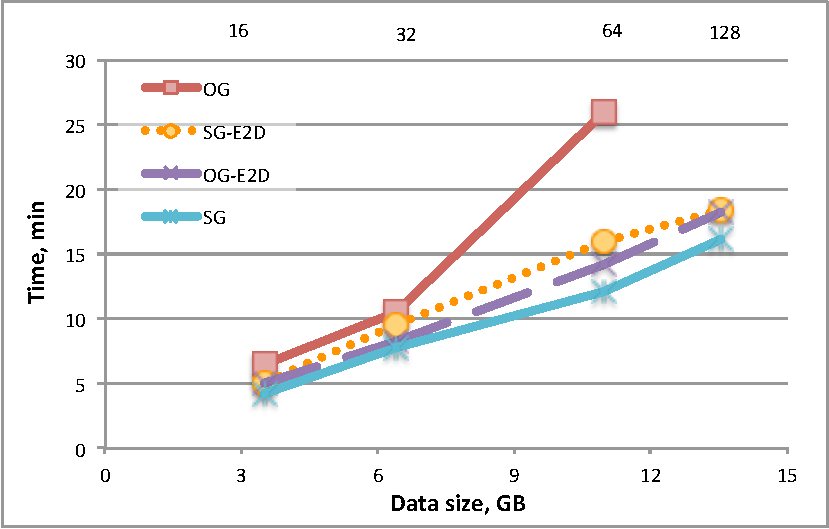
\includegraphics[width=2.6in]{figs/complexq.pdf}
  \vspace{-0.1in}
\caption{\insql{TGroup}, PageRank, trend.}
\label{fig:complexq}
  \vspace{-0.1in}
\end{minipage}
\end{figure*}

E2D partitioning leads to performance improvements in all data
structures except MGC.

\subsection{\insql{TSelect} with \insql{trend(pagerank())}}

All the experiments so far evaluated performance of individual \ql
operations. We conclude this section with a cold-start execution of
the query:

\begin{small}
\begin{verbatim}
      Select vid, pr
      From (TSelect Any V[vid, trend(prank) as pr]
                    Any E
            From (TSelect All V[vid, pagerank() as prank]; 
                          All E
                  From nGrams
                  TWhere Start >= x And End <= y
                  TGroup by 8 years)
            TGroup by size).toVerticesFlat()
      Order by pr
      Limit 10
\end{verbatim}
\end{small}

As we saw above, SG outperforms other representations for data load
and for PageRank, while OGC is very efficient for temporal
aggregation.  This query combines all of these operations, and adds a
trend analytic, and a transformation of the vertices of the result
into a flat vertex relation.

SG with no partitioning, and OGC with E2D show comparable
performances, as seen in Figure~\ref{fig:complexq}.

\eat{
\begin{figure}[t]
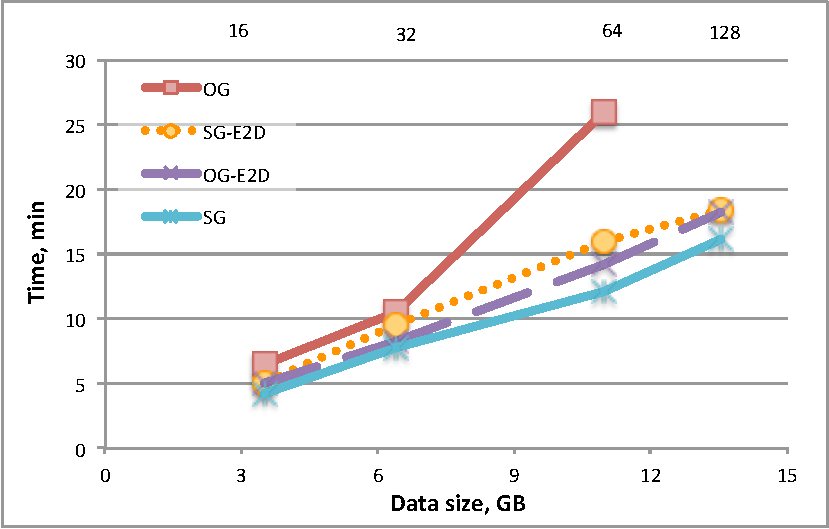
\includegraphics[width=3.2in]{figs/complexq.pdf}
\caption{Complex query: \insql{TGroup}, PageRank, trend.}
\label{fig:complexq}
\end{figure}
}

{\bf In summary,} no one data structure is most efficient across all
operations.  SG is most efficient for data load, because our file
format favors this data structure, and for PageRank.  OGC is most
efficient for temporal group and join.  The two data structures
perform comparably for the complex query.  E2D is the most efficient
partitioning method in most cases, and E2D-Temporal is a close second.
